\section{Task 1}
\FloatBarrier % Now figures cannot float above section title


\subsection{How original and unique is the designed robot?}


After discussion and doing some references, our group decide to make our robot arm as a four-arm robot and define the robot arms and joints, because there are some advantages of four-arm robot: better accuracy and stability of the movement; bigger working arrangement; better loading allowance; better collaboration.

\textbf{And there are also some unique assessments of our four-robot arms can meet:}
\begin{itemize}
    \item The welding robot arm allows for more precise control of welding position and angle.
    \item Compared to manual welding, welding robots can automate welding work, thereby increasing productivity and reducing labor costs.
    \item To prevent clashes between arms and joints, we perform kinematic analysis to determine the minimum spacing and range of movement between joints and robot arms, and use MATLAB simulations to ensure collision-free operation with exact arm and joint parameters.
    \item After researching robot design, we consider working arrangement, stability, and operability. To achieve precise welding in a specific area, we define parameters for all arms and joints.
\end{itemize}

\subsection{Property of all the arms and the joints}

We have designed 4 joints for the robot, 2 of which are revolute type and 2 are prismatic type. At the same time, there are four corresponding robotic arms, whose parameters are shown in the Table \ref{T 2.1} and Table \ref{T 2.2}

\begin{minipage}[htbp]{\textwidth}
    \makeatletter\def\@captype{table}
    \centering
    \scalebox{1}{
    \begin{tabular}{cccc}
    \hline
    Name & Body Mass (kg) & Center of mass & Inertia ($I_{xx}$ $I_{yy}$ $I_{zz}$) ($kg \cdot m^2$)                  \\ \hline
    R1   & 10        & (0 0 0)        & (0.27 0.27 0.8 )     \\
    R2   & 10        & (0 0 0)        & (0.27 0.27 0.8 )     \\
    P1   & 1.5       & (0 0 0)        & (0.07 0.07 0.07 )    \\
    P2   & 1.5       & (0 0 0)        & (0.07 0.07 0.07 )    \\
    Tool & 1.2       & (0 0 0)        & (0.002 0.002 0.004 ) \\ \hline
    \end{tabular}} 
    \caption{Experiment parameters}
    \label{T 2.1} 
\end{minipage}


\begin{minipage}[htbp]{\textwidth}
    \makeatletter\def\@captype{table}
    \centering
    \scalebox{1}{
    \begin{tabular}{cccc}
    \hline
    Joint & Type & Position Limit (rad \& m) & Joint Axis                   \\ \hline
    1   & revolute       & $[-5\frac{\pi}{180}, 5\frac{\pi}{180}]$ & [0 0 1]     \\
    2   & revolute       & $[-30\frac{\pi}{180}, 30\frac{\pi}{180}]$        & [0 1 0]     \\
    3   & prismatic      & $[-0.5,0.5]$        & [1 0 0]    \\
    4   & prismatic      & $[-1, 1]$        & [0 1 0]    \\ 
    Fixed &revolute & N/A & N/A \\\hline
    \end{tabular}} 
    \caption{Experiment parameters}
    \label{T 2.2} 
\end{minipage}

Figure \ref{F 2.1} is a schematic diagram of the robot in MATLAB.

\begin{figure}[htbp]
    \centering
    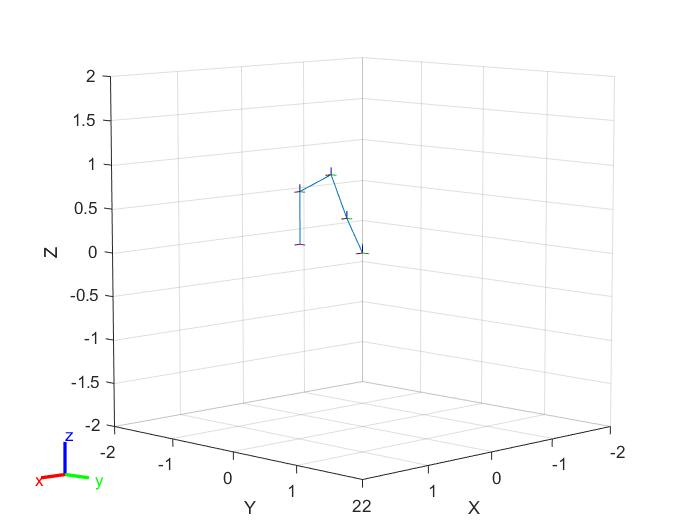
\includegraphics[width=7cm]{./fig/1.jpg}
    \caption{Force vs deformation and total moment diagram}
    \label{F 2.1}
\end{figure}

\subsection{Collision discussion}

Our designed robot is free from collisions. In most cases, collisions occur on the two arms of the rotating joints whose rotation angle is greater than $±90^\circ$. For our designed robot, the total range of motion for the two movable joints is $±35^\circ$, so there is no collision. Additionally, the animation of the robot's movement trajectory can be viewed in the dynamic image in Figure 8.
